\documentclass[11pt]{article}
\usepackage[nohead,margin=1.50in]{geometry} %set margins
\usepackage{amsmath,amssymb,amsthm,pdiag} %AMS packages for math stuff
\usepackage{multicol} % for use in HW section
\usepackage{graphicx}
\usepackage{enumitem}
  \setlist{topsep=1pt,itemsep=0pt,parsep=1pt}
  \setenumerate[1]{label=(\alph*)}

\newenvironment{problems}
{
 \begin{enumerate}[topsep=1pt,itemsep=0pt,parsep=2pt,%
 label={\arabic*.}, ref=\arabic*] \small
}
{
 \end{enumerate}
}

%%% Define some theorem and example environments. The starred versions
%%% are un-numbered and the unstarred versions are numbered.
\newtheoremstyle{plain}
  {\topsep}   % ABOVESPACE
  {\topsep}   % BELOWSPACE
  {\slshape}  % BODYFONT
  {0pt}       % INDENT (empty value is the same as 0pt)
  {\bfseries} % HEADFONT
  {.}         % HEADPUNCT
  {5pt plus 1pt minus 1pt} % HEADSPACE
  {}          % CUSTOM-HEAD-SPEC

\swapnumbers
\newtheorem{thm}{Theorem}[section]
\newtheorem{lem}[thm]{Lemma}
\newtheorem{prop}[thm]{Proposition}
\newtheorem{cor}[thm]{Corollary}
\newtheorem*{thm*}{Theorem}
\newtheorem*{lem*}{Lemma}
\newtheorem*{prop*}{Proposition}
\newtheorem*{cor*}{Corollary}

\theoremstyle{definition}
\newtheorem{defn}[thm]{Definition}
\newtheorem{example}[thm]{Example}
\newtheorem{examples}[thm]{Examples}
\newtheorem{rmk}[thm]{Remark}
\newtheorem{rmks}[thm]{Remarks}
\newtheorem{conv}[thm]{Convention}
\newtheorem*{defn*}{Definition}
\newtheorem*{example*}{Example}
\newtheorem*{examples*}{Examples}
\newtheorem*{rmk*}{Remark}
\newtheorem{rmks*}{Remarks}
\newtheorem*{conv*}{Convention}

%%% Define some convenient abbreviations for common mathematical
%%% notations.
\newcommand{\R}{\mathbb{R}} % use \R for the real numbers
\newcommand{\C}{\mathbb{C}} % use \C for the complex numbers
\newcommand{\Z}{\mathbb{Z}} % use \Z for the integers
\newcommand{\Q}{\mathbb{Q}} % use \Q for the rationals
\newcommand{\N}{\mathbb{N}} % use \N for the natural numbers
\newcommand{\F}{{\mathbb F}}
\newcommand{\compose}{\circ} % functional composition
\renewcommand{\implies}{\Rightarrow}
\renewcommand{\iff}{\Leftrightarrow}
\newcommand{\gen}[1]{\langle #1 \rangle}
\newcommand{\End}{\operatorname{End}}
\newcommand{\GL}{\mathrm{GL}}
\newcommand{\SL}{\mathrm{SL}}
\newcommand{\Orth}{\mathrm{O}}
\newcommand{\SO}{\mathrm{SO}}
\newcommand{\U}{\mathrm{U}}
\newcommand{\SU}{\mathrm{SU}}
\newcommand{\g}{\mathfrak{g}}
\newcommand{\transpose}{\mathsf{T}}
\newcommand{\B}{\mathcal{B}}
\newcommand{\Rep}{\operatorname{Rep}}
\newcommand{\Mat}{\operatorname{Mat}}
\newcommand{\inner}[2]{\langle #1, #2 \rangle}
\newcommand{\sgn}{\operatorname{sgn}}
\newcommand{\n}{\underline{\mathbf{n}}}
\newcommand{\Sym}{\mathbb{S}}
\newcommand{\Alt}{\mathbb{A}}
\newcommand{\D}{\mathbb{D}}
\newenvironment{perm}[2]{\left(\begin{smallmatrix}#1 \\ #2}{\end{smallmatrix}\right)}
\newcommand{\lcm}{\operatorname{lcm}}
\newcommand{\res}{\operatorname{res}}

\allowdisplaybreaks
\parskip=2pt

%\title{Document Title}
%\author{author's name}

\begin{document}%\maketitle
\setcounter{section}{13}


\section{Matrix groups}\noindent
Now we investigate groups formed by sets of matrices. These groups are
often infinite sets, so we will now be considering infinite groups, in
contrast to the finite groups we have seen so far. Initially, all of
our matrices will have real number entries.

\begin{defn}\index{matrix group}
  A \emph{group of matrices} (or \emph{matrix group} for short) is any
  nonempty set $G$ of $n \times n$ nonsingular matrices which is:
  \begin{enumerate}
  \item closed under products: for all $A,B \in G$, the product $AB
    \in G$.
  \item closed under inverses: for all $A \in G$, the inverse $A^{-1}
    \in G$.
  \end{enumerate}
\end{defn}

We only consider square $(n \times n$) matrices.  We have to restrict
to nonsingular matrices because we want our matrices to have
inverses. Recall that a basic theorem of linear algebra states that
\emph{a matrix is invertible if and only if it is nonsingular.} Recall
also that \emph{a matrix is nonsingular if and only if its determinant
  is nonzero.}

\begin{examples}
Here are some important examples of matrix groups. 

1. The \emph{general linear group}\index{general~linear~group}
$\GL(n)$\index{GL@$\GL(n)$} is the group consisting of all $n \times
n$ nonsingular matrices. In symbols,
\[
  \GL(n) = \{ n \times n \text{ matrices } A : \det A \ne 0\}.
\]
The group $\GL(n)$ is infinite (the cardinality of the set is
infinite). Note that $\GL(1)$ can be identified with the set
$\R^\times$ of units in $\R$, because the invertible $1 \times 1$
matrices are all of the form $[a]$ for $a \ne 0$.

2. The \emph{special linear group}\index{special~linear~group}
$\SL(n)$\index{SL@$\SL(n)$} is the group consisting of all $n \times
n$ matrices of determinant equal to $1$. In symbols,
\[
  \SL(n) = \{ A \in \GL(n) : \det A = 1 \}.
\]
By definition, we have an inclusion $\SL(n) \subset \GL(n)$. It is an
exercise to verify that this is a matrix group. Note that $\SL(1)$ is
actually a finite group, even though $\SL(n)$ is infinite, for all $n >
1$.

3. The \emph{orthogonal group}\index{orthogonal~group}
$\Orth(n)$\index{O@$\Orth(n)$} is the group consisting of all $n
\times n$ orthogonal matrices. A matrix $A$ is said to be an
\emph{orthogonal} matrix\index{orthogonal~matrix} if its inverse is
equal to its transpose: $A^{-1} = A^\transpose$. So, in symbols:
\[
  \Orth(n) = \{ A \in \GL(n) : A^{-1} = A^\transpose \}.
\]
It is an exercise to verify that this is a matrix group. Note that
$|\Orth(1)| = 2$. For all $n \ge 2$, the group $\Orth(n)$ is infinite.

4. The \emph{special orthogonal group}\index{special~orthogonal~group}
$\SO(n)$\index{SO@$\SO(n)$} is the group of all $n \times n$
orthogonal matrices of determinant equal to 1. In symbols,
\[
  \SO(n) = \{ A \in \Orth(n) : \det A = 1 \}.
\]
An orthogonal matrix of determinant 1 is also known as a \emph{proper}
orthogonal matrix\index{proper~orthogonal~matrix}. So we can rephrase
the definition to say: $\SO(n)$ is the group of all proper orthogonal
$n \times n$ matrices. Note that $\SO(1) = \SL(1)$ has a single
element, but $\SO(n)$ is infinite for all $n \ge 2$.
\end{examples}

\begin{rmk}\index{linear~group}
  Matrix groups are also called \emph{linear groups}. This is due to
  the fact that square matrices represent linear operators. If $A$ is
  an $n \times n$ matrix, then the function $\alpha: \R^n \to \R^n$
  defined by $\alpha(X) = AX$ is a linear operator. So every matrix
  group is isomorphic to a group of linear operators.
\end{rmk}

We will use some basic linear algebra to find a nice set of generators
for the group $\GL(n)$. Recall that \emph{elementary row operations}
are used to solve systems of linear equations (by Gaussian
elimination). The elementary row operations on a matrix are:
\begin{enumerate}[label=(\roman*),leftmargin=1in]
 \item add $t$ times row $j$ to row $i$, for any $i \ne j$, any $t \in \R$,
 \item multiply row $i$ by a scalar $t \in \R$, for any $i$, any $t \ne 0$, 
 \item swap row $i$ and row $j$, for any $i \ne j$.
\end{enumerate}
If $A$ is a matrix, then the elementary row operations on $A$ are
equivalent to  left multiplication of $A$ by the appropriate
corresponding elementary matrix. The elementary matrices are denoted
by:
\begin{enumerate}[label=(\roman*),leftmargin=1in]
 \item $E_{ij}(t)$, for any $i \ne j$, any $t \in \R$,
 \item $M_{i}(t)$, for any $i$, any $t \ne 0$, 
 \item $P_{ij}$, for any $i \ne j$.
\end{enumerate}
By definition, the elementary matrices\index{elementary~matrix} are
precisely those matrices that are obtained from an identity matrix by
performing a single elementary row operation of the corresponding
type. This rule defines a bijection from elementary row operations
onto elementary matrices.

\begin{thm}
  If $A$ is any $n \times n$ matrix and $B$ is the matrix resulting
  from performing a single elementary row operation to $A$ then $B =
  UA$, where $U$ is the corresponding elementary matrix of the same
  type.
\end{thm}

This simple result is proved in most linear algebra textbooks. The
proof is an easy calculation. The theorem has the following pleasant
consequence.

\begin{cor}
  Any nonsingular $n \times n$ matrix $A$ can be expressed as a product
  of elementary matrices.
\end{cor}

\begin{proof}
The proof is constructive: it tells us not only that the desired
factorization exists, it also gives an algorithm that we may use to
find one. 

Let $A$ be a nonsingular $n \times n$ matrix. Then the reduced echelon
form of $A$ is $I$, so by applying Gaussian elimination to $A$ we can
row reduce $A$ to $I$. This means that there is a finite sequence of
elementary row operations that transform $A$ to $I$. Let $U_1, U_2,
\dots, U_k$ be the elementary matrices corresponding to the elementary
row operations, in order. Then by the theorem, we have 
\[
  I = (U_k U_{k-1} \cdots U_2 U_1) A.
\]
It follows by matrix algebra that $A = U_1^{-1} U_2^{-1} \cdots
U_{k-1}^{-1} U_k^{-1}$. Since the inverse of any elementary matrix is
another elementary matrix of the same type, we are finished.
\end{proof}

The corollary gives us a nice set of generators for the general linear
group $\GL(n)$. Before we formulate the result, we make a formal
definition.

 
\begin{defn}\index{generators}
In general, we say that a group $G$ is \emph{generated} by a set $S
\subset G$ of its elements if every element of $G$ is expressible as a
product of elements of $S$ and inverses of elements of $S$.
\end{defn}

Now here is the result.

\begin{thm}
  The group $\GL(n)$ is generated by the set of $n \times n$
  elementary matrices.
\end{thm}

\begin{proof}
This follows immediately from the preceding corollary, which states
that any matrix in $\GL(n)$ is expressible as a product of elementary
matrices.
\end{proof}


\begin{rmk}
In general, to \emph{understand} a group, it is desirable to find a
nice subset of generators. Finding a set of generators reduces many
questions about the group to questions about its generators.

We have previously proved that the group $\Sym_n$ is generated by its
transpositions. This is a case in point: many questions about
permutations reduce to a question about transpositions. So too for the
matrix group $\GL(n)$: many questions about nonsingular matrices
reduce to a question about elementary matrices.

It should be emphasized that \emph{generating sets are not
  unique}. There are many different sets generating $\GL(n)$; the same
is true of $\Sym_n$.
\end{rmk}

\subsection*{Matrix groups are symmetry groups}\noindent
The groups introduced in this section are also symmetry groups. To see
this, recall that an $n \times n$ matrix $A$ represents the linear
operator $\alpha: \R^n \to \R^n$ defined by the rule $\alpha(X) =
AX$. Nonsingular matrices represent linear \emph{automorphisms}, the
bijective linear operators. So 
\[
  \GL(n) = \text{ the group of linear automorphisms of } \R^n.
\]
This is the symmetry group of the vector space $\R^n$, because the
linear automorphisms preserve the vector space structure.

The special linear group $\SL(n)$ is the group of linear automorphisms
of $\R^n$ preserving volume and orientation, in an appropriate
sense. To understand this, recall the following fact from
multivariable calculus: given three column vectors $P=(p_1, p_2,
p_3)$, $Q=(q_1, q_2, q_3)$, $R=(r_1, r_2, r_3) \in \R^3$, the absolute
value of the determinant of the $3 \times 3$ matrix $M = [P|Q|R]$ they
form gives the volume of the parallelopiped they generate, and the
sign of the determinant determines its orientation in some appropriate
sense. Then a linear operator $\alpha: \R^n \to \R^n$, given by the
rule $\alpha(X) = AX$ with $A$ a $3 \times 3$ matrix, is volume and
orientation preserving if and only if the determinant of $M$ remains
unchanged when we replace the vectors $P, Q, R$ by $\alpha(P),
\alpha(Q), \alpha(R)$. Equivalently, $\alpha$ preserves volume and
orientation if and only if $\det M = \det AM$, where $A$ represents
$\alpha$. This is equivalent to $\det A = 1$. That explains the idea
for $\R^3$, and it turns out that this can be (with a fair amount of
work) extended to $\R^n$ for any $n$.

The orthogonal group $\Orth(n)$ is the group of linear automorphisms
of $\R^n$ preserving the usual dot product. Since dot product
determines length and angle, we can also say that $\Orth(n)$ is the
group of linear automorphisms of $\R^n$ preserving length and angle,
but it is simpler to focus on the dot product. A linear operator
$\alpha: \R^n \to \R^n$ is given by the rule $\alpha(X) = AX$, where
$A$ is a matrix. If for any pair $X,Y$ of vectors in $\R^n$ we have
\[
  \alpha(X) \cdot \alpha(Y) = X \cdot Y 
\]
then we say that the operator $\alpha$ preserves the dot
product. Recall that the dot product of two column vectors may also be
written as a matrix product: $X \cdot Y = X^\transpose Y$. Thus, the
above dot product equality is equivalent to the following:
\[
  (AX)^\transpose (AY) = X^\transpose Y \iff X^\transpose A^\transpose
A Y = X^\transpose Y.
\]
Since this condition has to hold for all $X,Y \in \R^n$, it follows
that it holds if and only if $A^\transpose A = I$, which is equivalent
to the condition $A^{-1} = A^\transpose$. So $\alpha$ preserves dot
product if and only if $A^{-1} = A^\transpose$.

From the last paragraph it is not hard to see that $\SO(n)$ is the
group of linear automorphisms of $\R^n$ which preserve volume,
orientation, and dot product (distance and angle).

We can only hint at the many beautiful and profound connections
between matrix groups and geometry. There are many books devoted
entirely to one or more aspects of this, so it is impossible to be
comprehensive here.


\section*{Exercises}
\begin{problems}
\item Recall that the determinant of a product of matrices equals the
  product of their determinants. Use this to prove that:
  \begin{enumerate}
  \item $\GL(n)$ is a matrix group.
  \item $\SL(n)$ is a matrix group. 
  \end{enumerate}

\item Prove that any matrix group $G$ must contain the identity matrix
  $I$.

\item Describe all the elements of $\SL(1)$. What is the order
  $|\SL(n)|$ of $\SL(n)$? Justify your answers.

\item Recall that the inverse of a product of two matrices is equal to
  the product of their inverses in reverse order: $(AB)^{-1} = B^{-1}
  A^{-1}$. The same is true of the transpose: $(AB)^\transpose =
  B^\transpose A^\transpose$. Use these facts to prove that $\Orth(n)$
  is a matrix group.

\item Prove that $|\Orth(1)| = 2$; i.e., $\Orth(1)$ is a group of order 2. 

\item Prove that $\Orth(n) = \{ A \in \GL(n) : AA^\transpose = I
  \}$. (Don't make the error of assuming that matrix multiplication is
  commutative.)

\item Suppose that an $n \times n$ orthogonal matrix $A = [A_1 | A_2 |
  \cdots |A_n]$ is regarded as a matrix of column vectors. 
  \begin{enumerate}
  \item Show that $A_i^\transpose A_j = \delta_{ij}$. (Here
    $\delta_{ij}$ is the \emph{Kronecker delta} symbol, defined to be
    1 if $i=j$ and $0$ otherwise.)
  \item Show that the dot product $A_i \cdot A_j = \delta_{ij}$.
  \item Deduce that if $i \ne j$ then $A_i \perp A_j$.
  \item Deduce that $|A_i| = 1$, i.e., $A_i$ is a unit vector for all
    $i$.
  \item Deduce that the columns of an $n \times n$ orthogonal matrix
    form an orthonormal basis of $\R^n$.
  \end{enumerate}
  

\item Prove that $\SO(n)$ is a matrix group. 

\item Prove that $\SO(1) = \SL(1)$ is a group of one element. 

\item Prove that $\SO(n) = \SL(n) \cap \Orth(n)$. [Hint: Show each
  side is a contained in the other.]

\item Prove that if $G, H \subset \GL(n)$ are any two matrix groups
  (consisting each of $n \times n$ matrices) then $G \cap H$ is
  another matrix group.

\item 
  \begin{enumerate}
  \item Prove that if $A \in \Orth(n)$ then $\det A = \pm 1$. 
  \item The matrices $A \in \Orth(n)$ of determinant $-1$ are called
    \emph{improper} orthogonal matrices. Is the set of improper
    orthogonal matrices a matrix group? Prove your answer.
  \end{enumerate}

\item Let $D(n)$ be the set of all diagonal matrices in $\GL(n)$. Show
  that $D(n)$ is a matrix group.

\item 
  \begin{enumerate}
  \item Prove that $E_{ij}(t) \in \SL(n)$, for any $i \ne j$, any $t
    \in \R$.
  \item Let $D_1(n)$ be the set of diagonal matrices in $\SL(n)$. Show
    that $D_1(n)$ is a matrix group. 
  \item ($*$) Prove that $\SL(n)$ is generated by the set $S = D_1(n)
    \cup \{ E_{ij}(t) : i \ne j,\ t \in \R \}$. [Hint: Argue that it
      is possible to row reduce any matrix $A \in \SL(n)$ to a
      diagonal matrix only using type (i) elementary row operations.]
  \end{enumerate}


\end{problems}



\newpage
\section{The group of rotations of the plane}\noindent
In this section we will look more closely at a special example, namely
the group $\SO(2)$. This is the group of all $2 \times 2$ orthogonal
matrices of determinant $1$.

What can be said about the matrices in $\SO(2)$? Let's figure out the
answer, which involves a calculation. Suppose that 
\[
  A = 
  \begin{bmatrix}
    a&b\\c&d
  \end{bmatrix}
  \in \SO(2).
\]
Then we know that $A^{-1} = A^\transpose$ and $\det A = 1$. The first
condition implies that $I = A^\transpose A$, which was obtained by
right multiplication by $A$. So we know that
\[
    \begin{bmatrix}
    a&c\\b&d
  \end{bmatrix}
    \begin{bmatrix}
    a&b\\c&d
  \end{bmatrix} = 
  \begin{bmatrix} 1&0\\0&1\end{bmatrix} .
\]
Equivalently, this says that 
\[
  \begin{bmatrix}
    a^2+c^2&ab+cd\\ab+cd&b^2+d^2
  \end{bmatrix} = 
  \begin{bmatrix} 1&0\\0&1\end{bmatrix} .
\]
In other words, the column vectors
$A_1 = [\begin{smallmatrix} a\\c \end{smallmatrix}]$,
$A_2 = [\begin{smallmatrix} b\\d \end{smallmatrix}]$ in the columns of
$A$ must have unit length, so they lie somewhere on the unit
circle. Also, the dot product $A_1 \cdot A_2 = ab+cd = 0$, so the
vectors $A_1, A_2$ are perpendicular. Since
$A_1 = [\begin{smallmatrix} a\\c \end{smallmatrix}]$ is on the unit
circle $x^2 + y^2 =1$, there must be some angle $\theta$ such that
$A_1 = [\begin{smallmatrix} \cos \theta \\ \sin
  \theta \end{smallmatrix}]$.
Since $A_1 \perp A_2$, the angle between $A_1$ and $A_2$ is $\pi/2$,
so
$A_2 = [\begin{smallmatrix} \cos(\theta+\pi/2) \\
  \sin(\theta+\pi/2) \end{smallmatrix}] = [\begin{smallmatrix} -\sin
  \theta \\ \cos \theta \end{smallmatrix}]$.
This proves that $A \in \SO(2)$ must be of the form
\[
A = R_\theta :=
\begin{bmatrix}
  \cos \theta & -\sin \theta \\ \sin \theta & \cos \theta
\end{bmatrix}
\]
for some real number $\theta$. Conversely, it is easy to check that
any matrix of the above form is in $\SO(2)$. This proves the following
result.

\begin{thm}
  The group $\SO(2)$ of all proper orthogonal $2 \times 2$ matrices is
  the group of all matrices of the form $R_\theta$, as defined
  above, where $\theta \in \R$.
\end{thm}

Because the trigonometric functions are periodic, with period $2\pi$,
it follows that $R_\theta = R_{\theta+2\pi}$. So in fact the set
$\SO(2)$ can be written more compactly as
\[
  \SO(2) = \{ R_\theta : \theta \in [0, 2\pi) \}.
\]
Regarded as linear operators on $\R^2$, a matrix $R_\theta \in
\SO(2)$ defines the function $\rho_\theta: \R^2 \to \R^2$ given by the
rule $\rho_\theta(X) = R_\theta X$. 

\begin{thm}\label{thm:rotation}
  The linear operator $\rho_\theta$ defined by $\rho_\theta(X) =
  R_\theta X$ is a rotation of $\R^2$ through $\theta$ radians, in the
  sense that if $X \in \R^2$ is regarded as a vector, then
  $Y=\rho_\theta(X)$ is the vector obtained by rotating $X$ through an
  angle of $\theta$ radians.
\end{thm}

\begin{proof}
Observe that the operation $\text{rot}_\theta$ of rotating the plane
by $\theta$ radians is a \emph{linear} operator on $\R^2$:
$\text{rot}_\theta(X_1 + X_2) = \text{rot}_\theta(X_1) +
\text{rot}_\theta(X_2)$ and $\text{rot}_\theta(cX) = c\,
\text{rot}_\theta(X)$ for all $c \in \R$, $X,X_1, X_2 \in \R^2$. Of
course, the function $\rho_\theta$ is also a linear operator. In
general, to prove equality of functions $f,g$, one must show that
$f(x) = g(x)$ for all $x$. But for linear transformations, showing
equality is easier, because it suffices to prove they agree on a basis
of the domain. So we only need to check that
\[
  \rho_\theta(\hat{\imath}) = \text{rot}_\theta(\hat{\imath}), \quad
  \rho_\theta(\hat{\jmath}) = \text{rot}_\theta(\hat{\jmath})
\]
where $\{ \hat{\imath}, \hat{\jmath} \} = \{ [\begin{smallmatrix}
  1\\0 \end{smallmatrix}],  [\begin{smallmatrix}
  0\\1 \end{smallmatrix}] \}$ is the standard basis of $\R^2$.
This verification is an exercise, and it completes the proof. 
\end{proof}

\begin{cor}\label{cor:rot-identities}
  We have $\rho_{\theta_1} \rho_{\theta_2} = \rho_{\theta_1+\theta_2}$
  and $(\rho_\theta)^{-1} = \rho_{-\theta}$. In particular, rotations
  commute: $\rho_{\theta_1} \rho_{\theta_2} = \rho_{\theta_2}
  \rho_{\theta_1}$ for all $\theta_1, \theta_2 \in \R$.
\end{cor}

\begin{proof}
This is clear from the fact that $\rho_\theta$ is a rotation. So
rotating by $\theta_2$ radians followed by rotating by $\theta_1$
radians is the same as rotating by $\theta_1+\theta_2$ radians, etc.
\end{proof}

This corollary immediately implies that we have similar relations on
the rotation matrices: 
\[
  R_{\theta_1} R_{\theta_2} = R_{\theta_1+\theta_2}
  \quad\text{and}\quad (R_\theta)^{-1} = R_{-\theta}.
\]
In particular, rotation matrices commute: $R_{\theta_1} R_{\theta_2} =
R_{\theta_2} R_{\theta_1}$ for all $\theta_1, \theta_2 \in \R$.


\begin{cor}
  The matrix group $\SO(2)$ is isomorphic to the group
  $\{ \rho_\theta : \theta \in \R \}$ of rotations of the euclidean
  plane $\R^2$.
\end{cor}

\begin{proof}
The isomorphism is given by $f(R_\theta) = \rho_\theta$. 
\end{proof}

Now we consider \emph{improper} orthogonal $2 \times 2$ matrices. By
definition, these are the matrices $A \in \Orth(2)$ of determinant
equal to $-1$. One such matrix is the matrix
\[
  H_0 = \begin{bmatrix}
    1&0\\0&-1
  \end{bmatrix}.
\]
The corresponding linear operator on $\R^2$ is defined by $X \mapsto
H_0X$; i.e., $(x,y) \mapsto (x,-y)$. Geometrically, this is the
operator of reflection across the horizontal axis. Now we can describe
all the improper orthogonal matrices in $\Orth(2)$; it turns out that
they are all reflections.


\begin{thm}\label{thm:improper-formula}
  (a) For any improper orthogonal $2 \times 2$ matrix $H$, the matrix
  product $H_0 H$ is a proper orthogonal matrix, i.e., $H_0 H \in
  \SO(2)$. The same holds for $HH_0$. 

  (b) Reflection $\text{refl}_\theta$ across the line through the
  origin at angle $\theta$ with the horizontal axis of $\R^2$ is a
  linear operator on $\R^2$, and its matrix $H_\theta$ is an improper
  orthogonal matrix.

  (c) $H_{\theta} = H_0 R_{-2\theta}$. 
\end{thm}

\begin{proof}
(a) Recall that for square matrices, the determinant of a product
  equals the product of the determinants.  Thus $\det(H_0H) =
  \det(H_0)\, \det(H) = (-1)(-1) = 1$. So $H_0 H \in \SO(2)$, as
  required. The other case is similar.

(b) It is easy to check that reflection is a linear operator. So we
  can represent $\text{refl}_\theta$ by some $2 \times 2$ matrix
  $H_\theta$ with respect to the standard basis of $\R^2$, so that
  $\text{refl}_\theta(X) = H_\theta X$, for all $X \in \R^2$.  Since
  the operator $\text{refl}_\theta$ preserves length of, and angles
  between, vectors, it is clear that $H_\theta \in
  \Orth(2)$. Furthermore, $\det(H_\theta) = -1$ because $H_\theta$
  cannot be a rotation.  So $H_\theta$ is an improper orthogonal
  matrix. By part (a), it follows that $H_0 H_\theta \in \SO(2)$;
  i.e., it is equal to some rotation matrix.

(c) It suffices to check that $H_0H_\theta = R_{-2\theta}$, because
  once we have that equation we can left multiply by $H_0$ (using
  $H_0^2 = I$) to obtain the result.  Since we know that $H_0H_\theta$
  is some rotation matrix, it is enough to look at what it does to a
  single chosen (nonzero) vector. Choose a point $P \ne 0$ on the line
  fixed by $\text{refl}_\theta$. Then $H_\theta P = P$ and $H_0
  H_\theta P = H_0P = P'$, where $P'$ is the reflection of $P$ across
  the horizontal axis. In the picture,
  \[
  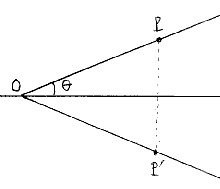
\includegraphics[scale=0.5]{angle.jpg}
  \]
  the angle $\angle POP'$ (where $O$ is the origin) is an angle of
  $-2\theta$ radians, so the effect of left multiplying by $H_0
  H_\theta$ is the same on $P$ as the effect of rotating $P$ by
  $-2\theta$ radians. So $H_0 H_\theta = R_{-2\theta}$, and we are
  done.
\end{proof}

In summary, we now have a complete understanding of the full
orthogonal group $\Orth(2)$. 


\begin{cor}
  $\Orth(2) = \{ R_\theta : \theta \in \R \} \cup \{ H_\theta :
  \theta \in \R\}$. 
\end{cor}

Another corollary of the theorem is that $\Orth(2)$ is generated by
$\SO(2)$ and $H_0$. (This is still true if $H_0$ is replaced by any
reflection.)

Now that we understand $\SO(2)$ and $\Orth(2)$, we return to the
dihedral groups $\D_n$ defined in a previous section. Recall that
\[
  \D_n = \{i, r, r^2, \dots, r^{n-1} \} \cup \{d, dr, dr^2, \dots,
  dr^{n-1} \}
\]
is the symmetry group of a regular $n$-gon. In the displayed
decomposition, the first set consists of rotations of the $n$-gon, and
the second consists of reflections of it. The reflection $d$ is the
one that fixes vertex $n$ of the $n$-gon.  

Note that all rotations and reflections of the $n$-gon must fix the
center point (centroid) of the $n$-gon. If we place the $n$-gon on the
euclidean plane $\R^2$ so that its centroid lies at the origin then
the rotations and reflections in $\D_n$ extend to rotations and
reflections of $\R^2$. (This requires further work to prove
rigorously, but it is intuitively clear.)

This means that the elements of the symmetry group $\D_n$ may be
represented by elements of the orthogonal group $\Orth(2)$; i.e., they
can be represented by $2 \times 2$ orthogonal matrices.  We choose to
place the $n$-gon in such a way that its $n$th vertex lies on the
positive $x$-axis. Then the extension of the symmetry $d$ is the
reflection $H_0$.  So the representation $f: \D_n \to \Orth(2)$ is
defined by
\[
  r \mapsto R_{2\pi/n}, \qquad d \mapsto H_0.
\]
The representation preserves products, in the sense that $f(ab) =
f(a)f(b)$, so the images displayed above determine the values of $f$
on every element of $\D_n$. Since $f$ is injective, it defines an
isomorphism of $\D_n$ onto the subgroup $\gen{R_{2\pi/n}, H_0}$ of
$\Orth(2)$ generated by $R_{2\pi/n}, H_0$.

So we can ``understand'' the dihedral group $\D_{n}$ by working with
matrices. 

What happens when we take the limit as $n$ approaches $\infty$? Well,
the regular $n$-gon approach a circle. The number of rotations, and
thus also the number of reflections, increases to infinity. So in some
sense it is fair to say that $\lim_{n \to \infty} \D_n =
\Orth(2)$. This enables another way to think of $\Orth(2)$ as a
symmetry group: $\Orth(2)$ is the symmetry group of a circle.  For
this reason, it is sometimes said that the group $\Orth(2)$ is the
``infinite dihedral group.''




\section*{Exercises}
\begin{problems}
\item Show that any matrix of the form $R_\theta$ must belong to
  $\SO(2)$, for any $\theta \in \R$.

\item Show that the origin is a fixed point for any rotation operator
  $\rho_\theta$.

\item Prove that the following identities follow from those in
  Corollary \ref{cor:rot-identities}.
  \begin{enumerate}
  \item $R_{\theta_1} R_{\theta_2} = R_{\theta_1+\theta_2}$
    and $(R_\theta)^{-1} = R_{-\theta}$, for all $\theta, \theta_1,
    \theta_2 \in \R$.
  \item $R_{\theta_1} R_{\theta_2} = R_{\theta_2} R_{\theta_1}$ for
    all $\theta_1, \theta_2 \in \R$.
  \end{enumerate}

\item Use the results of the preceding exercise to give a conceptual
  derivation of the addition formulas for sine and cosine.

\item Give a different proof of Theorem \ref{thm:rotation}, by showing
  that the angle between $X$ and $\rho_\theta(X)$ is equal to
  $\theta$, for any $0 \ne X\in \R^2$. [Hint: Recall that the angle
    between two vectors in $\R^2$ is determined by dot products.]

\item Show that the product of any two reflection matrices in
  $\Orth(2)$ must be a rotation matrix.

\item 
  \begin{enumerate}
  \item Show that $H_\theta = R_{2\theta} H_0$.
  \item Show that $R_{2\theta} H_0 R_{2\theta} = H_0$. What formula
    holding for dihedral groups is this similar to?
  \end{enumerate}

\item 
  \begin{enumerate}
  \item Argue that the composite of a reflection and a rotation (in
    either order) must be a reflection.
  \item Show that $H_{\theta_1} R_{\theta_2}$ must be some reflection
    matrix, i.e., some $H_{\theta_3}$. Figure out what reflection
    matrix it is; i.e., figure out how to express $\theta_3$ in terms
    of $\theta_1, \theta_2$. Justify your answer.
  \end{enumerate}

\end{problems}




\newpage
\section{Matrix groups over other fields}\noindent
Most of the basic theory of matrices, and indeed all of linear
algebra, which is usually developed initially over the field $\R$ of
real numbers, generalizes to any field\index{field} $F$. In this
generalization, the vector space $\R^n$ of $n$-tuples of real numbers
is replaced by the vector space $F^n$ of $n$-tuples over $F$, and
matrices with entries from $\R$ are replaced by matrices with entries
from $F$.

\begin{examples}
Here are some important examples of matrix groups over an arbitrary
field $F$. The field $F$ could be $\Q, \C$, or even a finite Galois
field $\F_p$.

1. The \emph{general linear group}\index{general~linear~group}
$\GL(n,F) = \GL_n(F)$\index{GL@$\GL_n(F)$} is the group consisting of
all $n \times n$ nonsingular matrices with entries from the field
$F$. In symbols,
\[
  \GL_n(F) = \{ n \times n \text{ matrices } A : \det A \ne 0\}.
\]
The group $\GL_n(F)$ is finite if the field $F$ is finite. 

2. The \emph{special linear group}\index{special~linear~group} $\SL(n,
F) = \SL_n(F)$\index{SL@$\SL_n(F)$} is the group consisting of all $n
\times n$ matrices of determinant equal to $1$. In symbols,
\[
  \SL_n(F) = \{ A \in \GL_n(F) : \det A = 1 \}.
\]
By definition, we have an inclusion $\SL_n(F) \subset
\GL_n(F)$. Again, this is a finite group if the field $F$ is finite.
\end{examples}

It is also possible to define orthogonal
groups\index{orthogonal~group} over fields other than $\R$, but there
are technicalities that we do not want to face at the moment.

When one allows the field $F$ to be the field of complex numbers, we
of course have $\GL_n(\C)$ and $\SL_n(\C)$ as above, but two important
extra examples appear, as follows.

\begin{examples}
1. The \emph{unitary group}\index{unitary~group} $\U(n) =
\U_n(\C)$\index{U@$\U(n)$} is the group consisting of all $n \times
n$ unitary matrices. A square matrix $A$ with complex entries is
\emph{unitary} if $A^{-1} = A^*$, where $A^* =
\overline{A}^\transpose$. The matrix $A^*$ is called the
\emph{conjugate transpose} of $A$. It is obtained by first taking the
complex conjugate of each entry of $A$ to get the matrix
$\overline{A}$, and then taking the transpose.

2. The \emph{special unitary group}\index{special~unitary~group}
$\SU(n) = \SU_n(\C)$\index{SU@$\SU(n)$} is the group consisting of all
$n \times n$ special unitary matrices. A square matrix $A$ with
complex entries is \emph{special unitary} if it is unitary and has
determinant equal to 1.
\end{examples}

Unitary groups play a fundamental role in mathematical physics. 


\begin{example}
Many basic properties of matrices work for matrices with entries from
an arbitrary ring $R$. This observation leads to many more new
examples of matrix groups.  For instance, the group
\[
  \SL(n,\Z) = \SL_n(\Z) = \{n \times n \text{ matrices $A$ with integer
    entries} \mid \det A = 1 \}
\]
makes sense and has been studied extensively. It is an example of an
\emph{arithmetic group}\index{arithmetic~group}. Arithmetic groups
have connections to number theory and lattice theory.
\end{example}

Lattice theory has recently been applied to invent new public-key
cryptosystems.



\section*{Exercises}\noindent

\begin{problems}
\item 
  \begin{enumerate}
  \item List all the matrices in $\GL_2(\F_2)$.
  \item List all the matrices in $\SL_2(\F_2)$.
  \end{enumerate}
 

\item Use counting principles to compute $|\GL_2(\F_p)|$. 

\item Use counting principles to compute $|\SL_2(\F_p)|$. 

\item Let $F$ be any field. Let $G$ be the set of all matrices of the
    form $E(t) = \begin{bmatrix} 1&t\\ 0&1
  \end{bmatrix}$, where $t \in F$. 
  \begin{enumerate}
  \item Show that $E(s) E(t) = E(s+t)$ for any
    $s,t \in F$.
  \item Show that $E(t)^{-1} = E(-t)$ for any $t \in F$.
  \item Prove that the set $G$ is a matrix group. (You have to show it
    is a nonempty set of matrices that is closed under products and
    inverses.)
  \end{enumerate}

\item Let $G$ be the set of all block matrices of the form
  $\begin{bmatrix} A&B\\ 0&C \end{bmatrix}$ with $A,B, C$ all $2\times
  2$ matrices over a field $F$ such that $\det(AC) \ne 0$. Verify that
  $G$ is a matrix group.

\item Show that $\SU(1) = \SU_1(\C)$ is isomorphic to the
  multiplicative group $\{ e^{i\theta} \mid \theta \in \R\}$ of points
  on the unit circle, regarded as a subgroup of $\C^\times$.

\end{problems}

\end{document}
